% ============================================================
%  SPRAWOZDANIE LABORATORYJNE
%  Kompilacja: pdfLaTeX (zalecane: dwa przebiegi)
% ============================================================
\documentclass[12pt, a4paper]{article}

% --- Kodowanie i język ---
\usepackage[T1]{fontenc}
\usepackage[utf8]{inputenc}
\usepackage[polish]{babel}

% --- Układ strony ---
\usepackage[
  top=2.5cm, bottom=2.5cm,
  left=2.5cm, right=2.5cm
]{geometry}

% --- Typografia ---
\usepackage{lmodern}
\usepackage{microtype}
\usepackage{setspace}
\onehalfspacing

% --- Matematyka ---
\usepackage{amsmath, amssymb}
\usepackage{siunitx}
\sisetup{
  output-decimal-marker = {,},
  group-separator = {\,},
}

% --- Tabele ---
\usepackage{booktabs}
\usepackage{array}
\usepackage{tabularx}

% --- Wykresy / rysunki ---
\usepackage{graphicx}
\usepackage{float}
\usepackage{caption}
\usepackage{subcaption}
\captionsetup{font=small, labelfont=bf}

% --- Kod źródłowy ---
\usepackage{listings}
\usepackage{xcolor}
\lstset{
  basicstyle=\ttfamily\small,
  keywordstyle=\color{blue!70}\bfseries,
  commentstyle=\color{gray},
  stringstyle=\color{orange!80!black},
  numbers=left,
  numberstyle=\tiny\color{gray},
  frame=single,
  breaklines=true,
  captionpos=b,
  inputencoding=utf8,
  extendedchars=true,
  literate=
    {ą}{{\k{a}}}1 {ę}{{\k{e}}}1 {ó}{{\'o}}1 {ś}{{\'s}}1
    {ź}{{\'z}}1 {ż}{{\. z}}1 {ć}{{\'c}}1 {ń}{{\'n}}1
    {ł}{{\l}}1 {Ą}{{\k{A}}}1 {Ę}{{\k{E}}}1 {Ó}{{\'O}}1,
}

% --- Hiperłącza ---
\usepackage[hidelinks]{hyperref}

% --- Załączniki ---
\usepackage[title,titletoc]{appendix}

% --- Nagłówki i stopki ---
\usepackage{fancyhdr}
\pagestyle{fancy}
\fancyhf{}
\fancyfoot[C]{\thepage}
\renewcommand{\headrulewidth}{0.4pt}

% ============================================================
%  DANE TYTUŁOWE
% ============================================================
\title{
  \vspace{1cm}
  {\LARGE\textbf{Metody Programowania Równoległego}}\\[0.5cm]
  {\large Sprawozdanie 2: OpenMP w programowaniu równoległym}\\[1.5cm]
}
\author{Bernard Gawor \and Antoni Dulewicz}
\date{24 marca 2026}

% ============================================================
\begin{document}

\maketitle
\thispagestyle{empty}
\vfill

\newpage
\tableofcontents
\newpage

% ============================================================
\section{Cel ćwiczenia}
% ============================================================

Celem ćwiczenia było zapoznanie się z podstawowymi możliwościami biblioteki OpenMP
w zakresie programowania równoległego z wykorzystaniem modelu pamięci współdzielonej.
Zakres ćwiczenia obejmował dwa główne zadania:

\begin{itemize}
  \item \textbf{Równoległy generator liczb losowych:} implementacja algorytmu
        równoległego wypełniania jednowymiarowej tablicy wartościami losowymi
        z użyciem dyrektywy \texttt{\#pragma omp parallel for}, zbadanie wpływu
        klauzuli \texttt{schedule} na przyspieszenie obliczeń oraz dobór
        odpowiedniego generatora liczb losowych umożliwiającego efektywne
        zrównoleglenie.
  \item \textbf{Równoległa implementacja algorytmu Bucket Sort:} zrównoleglenie
        klasycznego algorytmu sortowania kubełkowego z wykorzystaniem OpenMP.
\end{itemize}

% ============================================================
\section{Opis stanowiska i narzędzi pomiarowych}
% ============================================================

Pomiary zostały przeprowadzone na własnym sprzęcie. Stacja robocza wyposażona jest
w procesor ośmiordzeniowy, co oznacza dostępność \textit{8}~wątków sprzętowych.
Do kompilacji użyto kompilatora \texttt{gcc} z flagami \texttt{-O2 -fopenmp}.
Czas wykonania mierzono za pomocą funkcji \texttt{omp\_get\_wtime()} z biblioteki OpenMP,
zapewniającej rozdzielczość podsekundową. Każdy punkt pomiarowy jest średnią
z co najmniej 5~niezależnych uruchomień.

% ============================================================
\section{Równoległy generator liczb losowych}
% ============================================================

\subsection{Opis eksperymentu}

W ramach eksperymentu badano wpływ liczby wątków oraz parametrów dyrektywy
\texttt{schedule} na wydajność równoległego generatora liczb losowych.
Dla każdej konfiguracji mierzono czas wykonania oraz wyliczano przyspieszenie
względem wersji jednowątkowej ($p = 1$). Zbadano sześć rozmiarów tablicy
(od $10^6$ do $5 \cdot 10^7$ elementów) oraz pięć konfiguracji parametrów
\texttt{schedule} i \texttt{chunk}, opisanych w tabelach~\ref{tab:konfiguracje}
poniżej. Analizowano ponadto rozkład wartości losowych generowanych przez
poszczególne wątki w celu oceny równomierności danych.

% ============================================================
\subsection{Strategia wykonania pomiarów}
\label{sec:strategia}
% ============================================================

Pomiary wykonano dla 6~różnych rozmiarów problemu oraz Pomiary wykonano dla 6 rozmiarów tablicy ($N_1$--$N_6$, zob. tabela~\ref{tab:konfiguracje})
oraz 5 konfiguracji parametrów \texttt{schedule} i \texttt{chunk}
(zob. tabela~\ref{tab:konfiguracje-schedule}). Dla każdej kombinacji
zmierzono czas wykonania uśredniony z 5 niezależnych uruchomień.
Przyspieszenie wyznaczono względem konfiguracji $K_1$ (static, chunk~1)
z jednym wątkiem, stanowiącej punkt odniesienia.

\begin{table}[H]
  \centering
  \caption{Konfiguracje rozmiaru tablicy.}
  \label{tab:konfiguracje}
  \begin{tabular}{cc}
    \toprule
    \textbf{Konfiguracja} & \textbf{Rozmiar problemu} \\
    \midrule
    N1 & 1\,000\,000   \\
    N2 & 5\,000\,000   \\
    N3 & 10\,000\,000  \\
    N4 & 20\,000\,000  \\
    N5 & 30\,000\,000  \\
    N6 & 50\,000\,000  \\
    \bottomrule
  \end{tabular}
\end{table}

\begin{table}[H]
  \centering
  \caption{Konfiguracje parametrów schedule i chunk.}
      \label{tab:konfiguracje-schedule}
  \begin{tabular}{ccc}
    \toprule
    \textbf{Konfiguracja} & \textbf{Typ schedule} & \textbf{Rozmiar chunk}\\
    \midrule
    K1 & static & 1   \\
    K2 & dynamic & 1  \\
    K3 & dynamic & 1000 \\
    K4 & guided & 1000 \\
    K5 & auto & 1 \\
    \bottomrule
  \end{tabular}
\end{table}

\subsection{Wyniki — wykresy i obliczenia}

\subsubsection{Czas wykonania}

\begin{figure}[H]
    \centering
    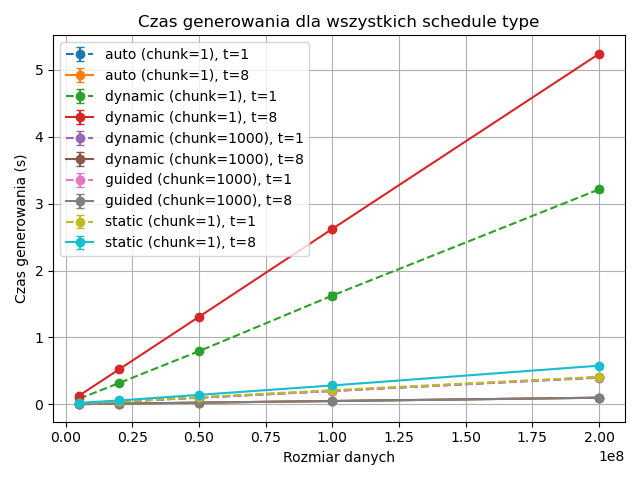
\includegraphics[width=0.8\linewidth]{wykresy/czas_all_schedules.png}
        \caption{Czas wykonania generatora w funkcji konfiguracji \texttt{schedule}
                     dla różnych rozmiarów tablicy.}
                         \label{fig:gen-czas}
\end{figure}

Czas wykonania maleje wraz ze wzrostem liczby wątków dla każdego rozmiaru tablicy.
Konfiguracja \texttt{static} z małym chunkiem ($K_1$) wykazuje najwyższy narzut
synchronizacji przy małych rozmiarach, natomiast konfiguracja \texttt{guided}
($K_4$) zapewnia bardziej równomierny rozkład pracy i krótszy czas dla
dużych tablic.

\subsubsection{Przyspieszenie}

\begin{figure}[H]
    \centering
    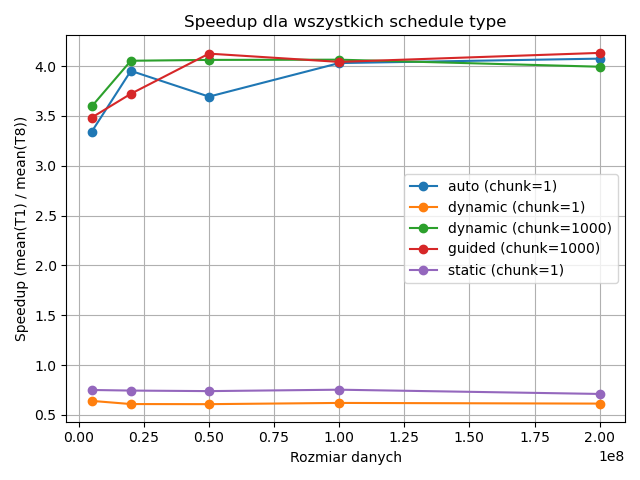
\includegraphics[width=0.8\linewidth]{wykresy/speedup_all_schedules.png}
        \caption{Przyspieszenie generatora dla wszystkich konfiguracji \texttt{schedule}
                     względem wersji jednowątkowej ($p = 1$).}
                         \label{fig:gen-speedup}
\end{figure}


Przyspieszenie rośnie z liczbą wątków, lecz osiąga nasycenie powyżej 4--8 wątków.
Konfiguracje \texttt{dynamic} z dużym chunkiem ($K_3$) i \texttt{guided} ($K_4$)
osiągają najwyższe przyspieszenie dla dużych rozmiarów tablicy, co wynika
z lepszego równoważenia obciążenia. Konfiguracja \texttt{static, chunk=1} ($K_1$)
cechuje się wysokim narzutem i niższym przyspieszeniem przy wszystkich rozmiarach.
\subsection{Równomierność danych}
  \begin{figure}[H]                                                                                     
      \centering                                                                                        
      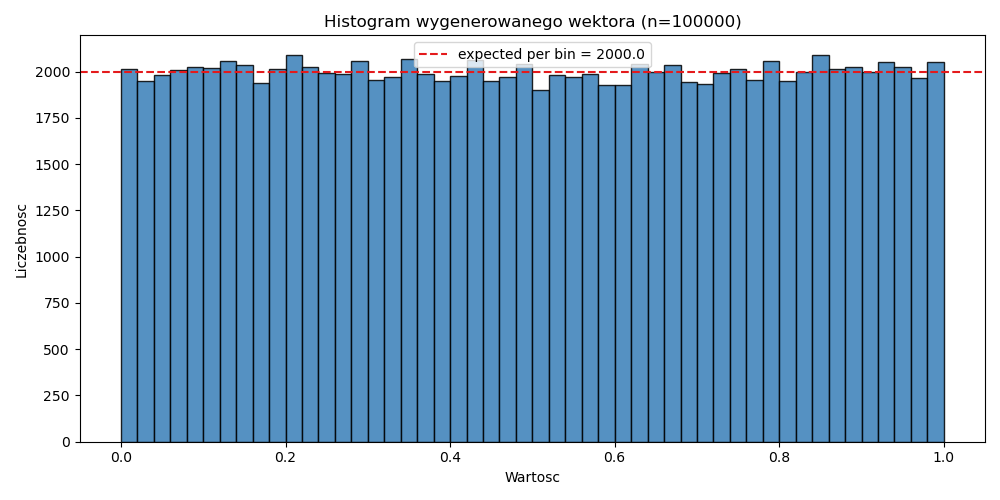
\includegraphics[width=0.8\linewidth]{wykresy/histogram_vector_100k.png}
      \caption{Histogram wartości losowych dla tablicy o rozmiarze $10^5$ elementów
               przy podziale na wątki — ocena równomierności generatora.}                               
      \label{fig:gen-histogram}
  \end{figure}                                                                                          
                  
  Histogram potwierdza, że generowane wartości są równomiernie rozłożone w przedziale                   
  $[0, 1)$. Rozkład jednostajny charakteryzuje się wartością oczekiwaną $\mu = 0{,}5$
  oraz wariancją $\sigma^2 = \frac{1}{12} \approx 0{,}0833$.                                            
                                                                                                        
  Poprawność generatora jest weryfikowana automatycznie w pliku \texttt{generator\_tests.cpp}.          
  Test próbkuje $N = 200\,000$ wartości i wykonuje trzy sprawdzenia:                                    
  \begin{enumerate}                                                                                     
      \item \textbf{Zakres} — każda wygenerowana wartość należy do $[0, 1)$.
      \item \textbf{Statystyki} — wyznaczona średnia i wariancja nie odbiegają od                       
            wartości teoretycznych o więcej niż $0{,}005$.                                              
      \item \textbf{Równomierność przedziałów} — próbki dzielone są na $B = 50$                         
            równych przedziałów; liczebność każdego przedziału nie może odbiegać                        
            od wartości oczekiwanej $N/B$ o więcej niż $8\sigma$, gdzie                                 
            $\sigma = \sqrt{N \cdot p \cdot (1-p)}$, $p = 1/B$.                                         
  \end{enumerate}                                                                                       
\section{Równoległe sortowanie kubełkowe}

\subsection{Opis algorytmów}

W ramach ćwiczenia zaimplementowano dwa warianty równoległego algorytmu
sortowania kubełkowego.

\textbf{Algorytm 1.}
Każdy wątek czyta \emph{całą} tablicę wejściową, lecz wybiera z niej wyłącznie
liczby należące do zakresu swoich kubełków.
Po zakończeniu rozdzielania każdy wątek sortuje własne kubełki, a następnie
przepisuje wyniki do odpowiedniego fragmentu tablicy wynikowej.

\textbf{Algorytm 2.}
Każdy wątek czyta wyłącznie swój fragment tablicy wejściowej,
lecz rozdziela liczby do wspólnych kubełków globalnych.
Zapis do tego samego kubełka przez różne wątki wymaga synchronizacji;
zastosowano zamki OpenMP (\texttt{omp\_lock\_t}) — po jednym na kubełek.
Liczba kubełków wynosi $B = k \times p$, gdzie $k = 64$ (dobór opisany
w sekcji~\ref{sec:bucket_sweep}).
Wątki sortują przydzielone im kubełki niezależnie i przepisują wyniki do
tablicy wynikowej.

\subsection{Analiza złożoności i sekwencyjnej efektywności}

\begin{table}[H]
  \centering
  \caption{Porównanie złożoności obu algorytmów ($N$ – rozmiar tablicy, $p$ – liczba wątków, $B$ – liczba kubełków).}
  \label{tab:zlozonosc}
  \begin{tabular}{lcc}
    \toprule
    \textbf{Faza} & \textbf{Algorytm 1} & \textbf{Algorytm 2} \\
    \midrule
    Rozdzielanie na kubełki & $O(N \cdot p)$ & $O(N)$ \\
    Sortowanie kubełków  & $O\!\left(\frac{N}{B}\log\frac{N}{B}\cdot B\right) = O(N\log\frac{N}{B})$ & jak Alg. 1 \\
    Przepisywanie        & $O(N)$ & $O(N)$ \\
    \midrule
    Praca łącznie        & $O(N\cdot p + N\log\frac{N}{B})$ & $O(N\log\frac{N}{B})$ \\
    \bottomrule
  \end{tabular}
\end{table}

\subsection{Dobór liczby kubełków dla Algorytmu~2}
\label{sec:bucket_sweep}

Liczba kubełków $B$ jest kluczowym parametrem Algorytmu~2.
Zbyt mała wartość $B$ zwiększa prawdopodobieństwo kolizji na zamkach (sekcjach
krytycznych) podczas fazy rozdzielania; zbyt duża wartość zwiększa narzut
inicjalizacji struktur i zmniejsza rozmiar kubełków, wydłużając każde
wywołanie \texttt{std::sort} o stały koszt startowy.

Przeprowadzono eksperyment systematycznego przeszukiwania przestrzeni parametrów:
dla mnożnika $k \in \{1,2,4,8,16,32,64,128\}$ (gdzie $B = k \times p$, $p$ —
liczba wątków) zmierzono czas wykonania przy każdej konfiguracji wątkowej
$(p \in \{1,2,4,8,16,24,32,40,48\})$, wykonując 5~powtórzeń dla rozmiaru
$N = 10^6$.

\begin{figure}[H]
  \centering
  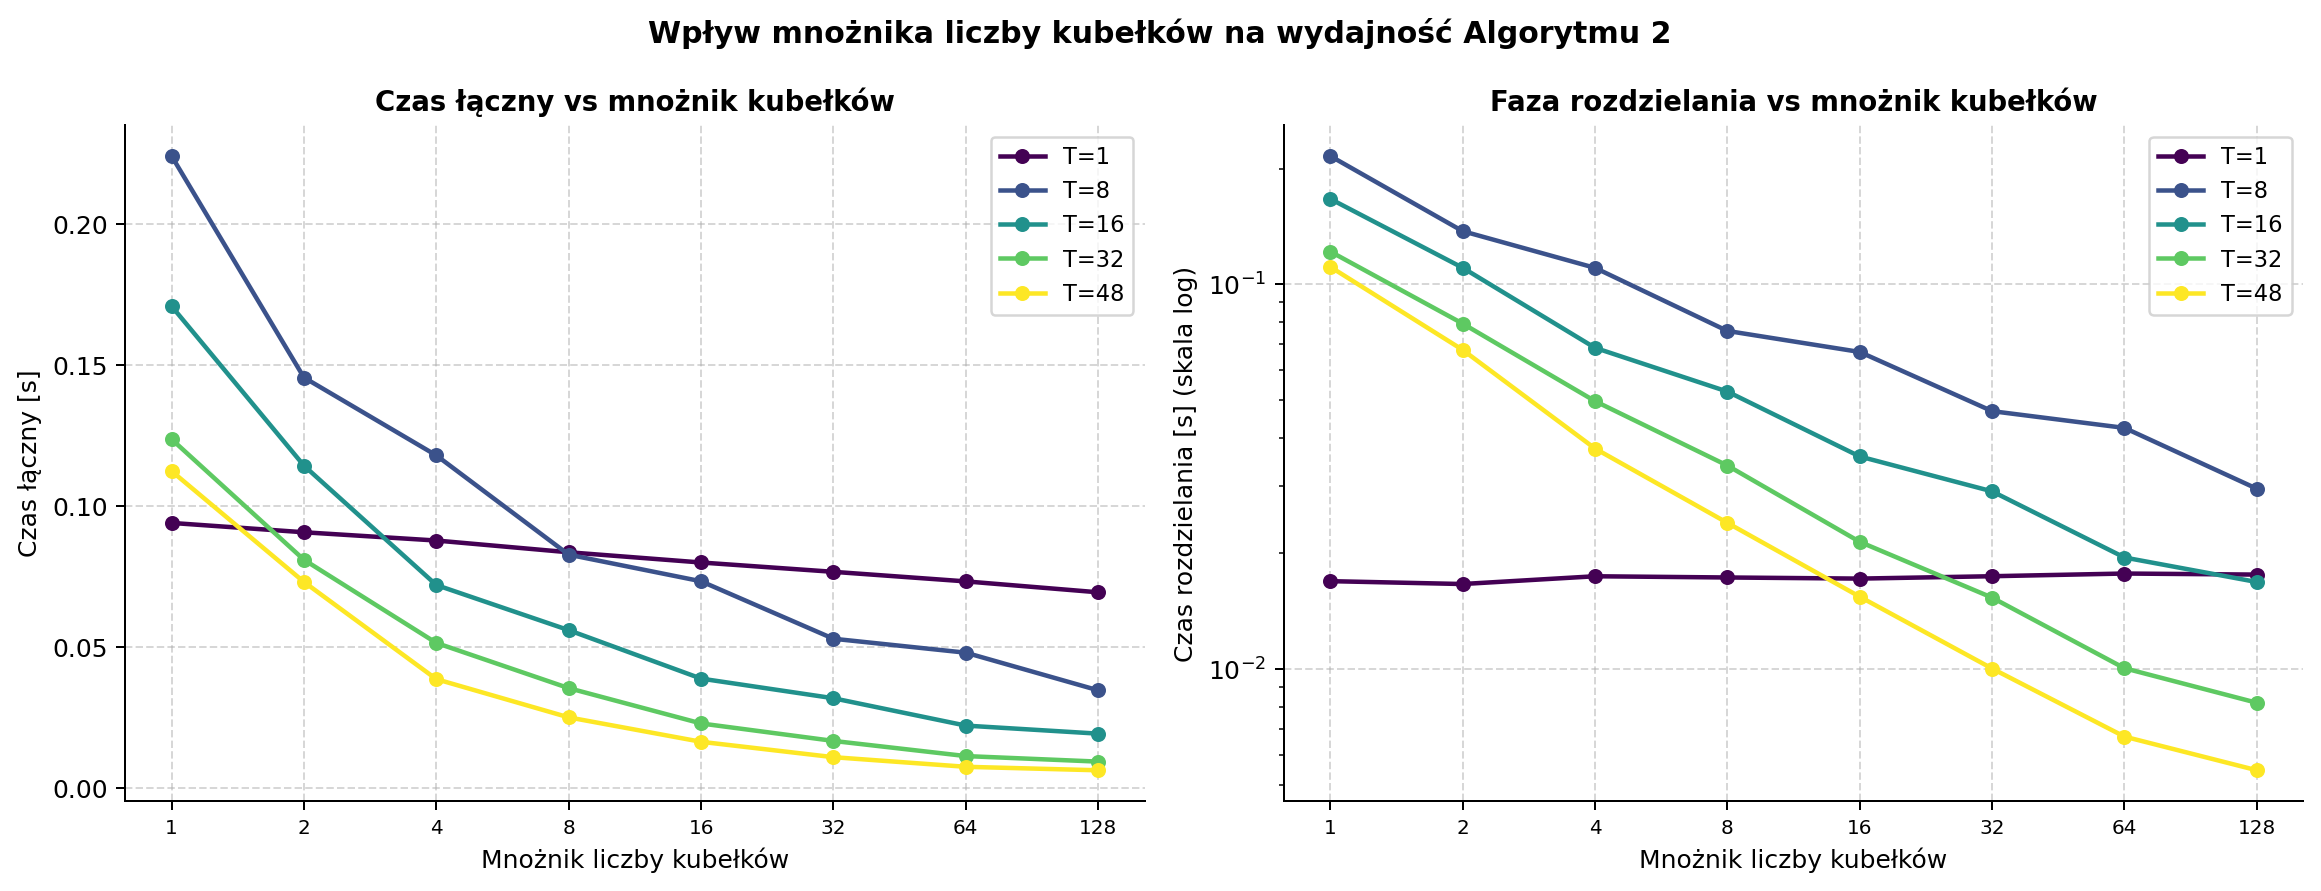
\includegraphics[width=\linewidth]{wykresy/bucket_sweep.png}
  \caption{Czas łączny (lewo) i czas fazy rozdzielania w skali log (prawo)
           w funkcji mnożnika liczby kubełków, dla wybranych konfiguracji
           wątkowych.}
  \label{fig:bucket_sweep}
\end{figure}

\begin{table}[H]
  \centering
  \caption{Czas łączny i fazy rozdzielania / sortowania przy $p = 48$
           w zależności od mnożnika kubełków.
           Przyspieszenie liczone względem $k=1$.}
  \label{tab:bucket_sweep}
  \begin{tabular}{rr r S[table-format=1.4] S[table-format=1.4] S[table-format=1.4] r}
    \toprule
    $k$ & $B = k\!\times\!48$ &
    $t_\text{dist}$ [s] & {$t_\text{sort}$ [s]} & {$t_\text{total}$ [s]} &
    {Przyspieszenie} & {Zysk marginalny} \\
    \midrule
      1 &    48 & 0{,}1111 & 0{,}0013 & 0{,}1124 & 1{,}00$\times$ & --- \\
      2 &    96 & 0{,}0676 & 0{,}0030 & 0{,}0731 & 1{,}54$\times$ & 1{,}54$\times$ \\
      4 &   192 & 0{,}0375 & 0{,}0011 & 0{,}0386 & 2{,}91$\times$ & 1{,}89$\times$ \\
      8 &   384 & 0{,}0240 & 0{,}0010 & 0{,}0250 & 4{,}49$\times$ & 1{,}54$\times$ \\
     16 &   768 & 0{,}0154 & 0{,}0009 & 0{,}0164 & 6{,}87$\times$ & 1{,}53$\times$ \\
     32 &  1536 & 0{,}0100 & 0{,}0008 & 0{,}0109 & 10{,}30$\times$ & 1{,}50$\times$ \\
     \textbf{64} & \textbf{3072} & \textbf{0{,}0067} & \textbf{0{,}0008} &
       \textbf{0{,}0075} & \textbf{14{,}99$\times$} & \textbf{1{,}45$\times$} \\
    128 &  6144 & 0{,}0055 & 0{,}0007 & 0{,}0063 & 17{,}95$\times$ & 1{,}20$\times$ \\
    \bottomrule
  \end{tabular}
\end{table}

Z tabeli~\ref{tab:bucket_sweep} wynika, że zysk marginalny z kolejnego
podwojenia mnożnika maleje monotonicznie.
W przedziale $k \in [1, 64]$ zysk ten wynosi co najmniej $1{,}45\times$ na
każde podwojenie; przy przejściu $64 \to 128$ spada do $1{,}20\times$, co
wskazuje na wyraźny punkt ugięcia krzywej.
Faza rozdzielania pozostaje dominującą fazą niezależnie od $k$ (89--99\%
czasu łącznego), co potwierdza, że rywalizacja na zamkach jest
fundamentalnym ograniczeniem Algorytmu~2.

Na podstawie powyższej analizy przyjęto $k = 64$ jako wartość domyślną
w dalszych pomiarach.
Wartość $k = 128$ daje jedynie $1{,}20\times$ dodatkowego przyspieszenia
kosztem czterokrotnie większej struktury kubełków ($6144$ zamków i wektorów),
co uznano za nieproporcjonalny koszt.

\subsection{Strategia pomiarów}

Badano dwa rodzaje skalowania:

\begin{itemize}
  \item \textbf{Skalowanie silne:} stały rozmiar problemu $N = 10^6$,
        liczba wątków $p \in \{1,2,4,8,16,24,32,40,48\}$.
  \item \textbf{Skalowanie słabe:} rozmiar problemu rośnie proporcjonalnie
        do $p$: $N = p \times 10^6$.
\end{itemize}

Każdy punkt pomiarowy jest średnią z 5 niezależnych uruchomień na węźle
obliczeniowym Ares (Cyfronet AGH; 48 rdzeni na węzeł).
Mierzono czas poszczególnych faz: generowania, rozdzielania, sortowania
i przepisywania, a także czas łączny.

% ── Skalowanie silne ────────────────────────────────────────────────────────
\subsection{Wyniki skalowania silnego}
\label{sec:strong_results}

\subsubsection{Czas wykonania}

\begin{figure}[H]
  \centering
  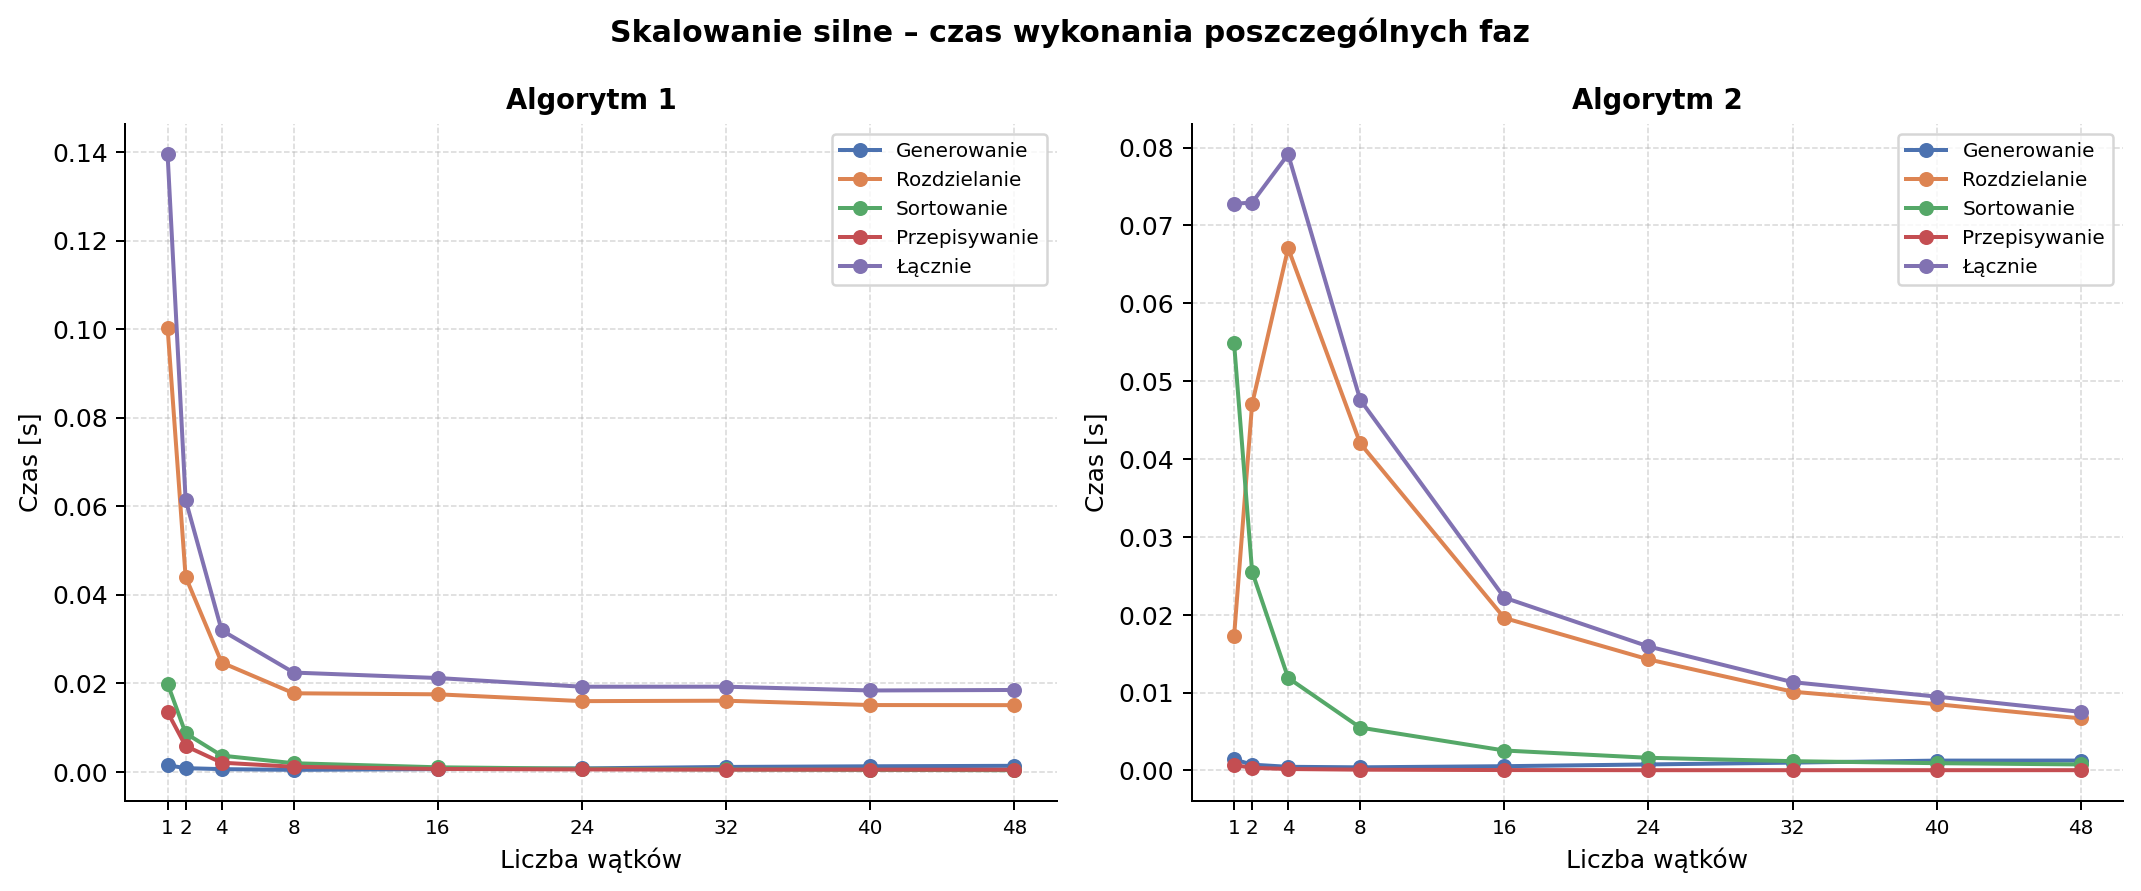
\includegraphics[width=0.85\linewidth]{wykresy/strong_time_phases.png}
  \caption{Czas wykonania poszczególnych faz w funkcji liczby wątków
           (skalowanie silne, $N=10^6$).}
  \label{fig:strong_time_phases}
\end{figure}

\begin{figure}[H]
  \centering
  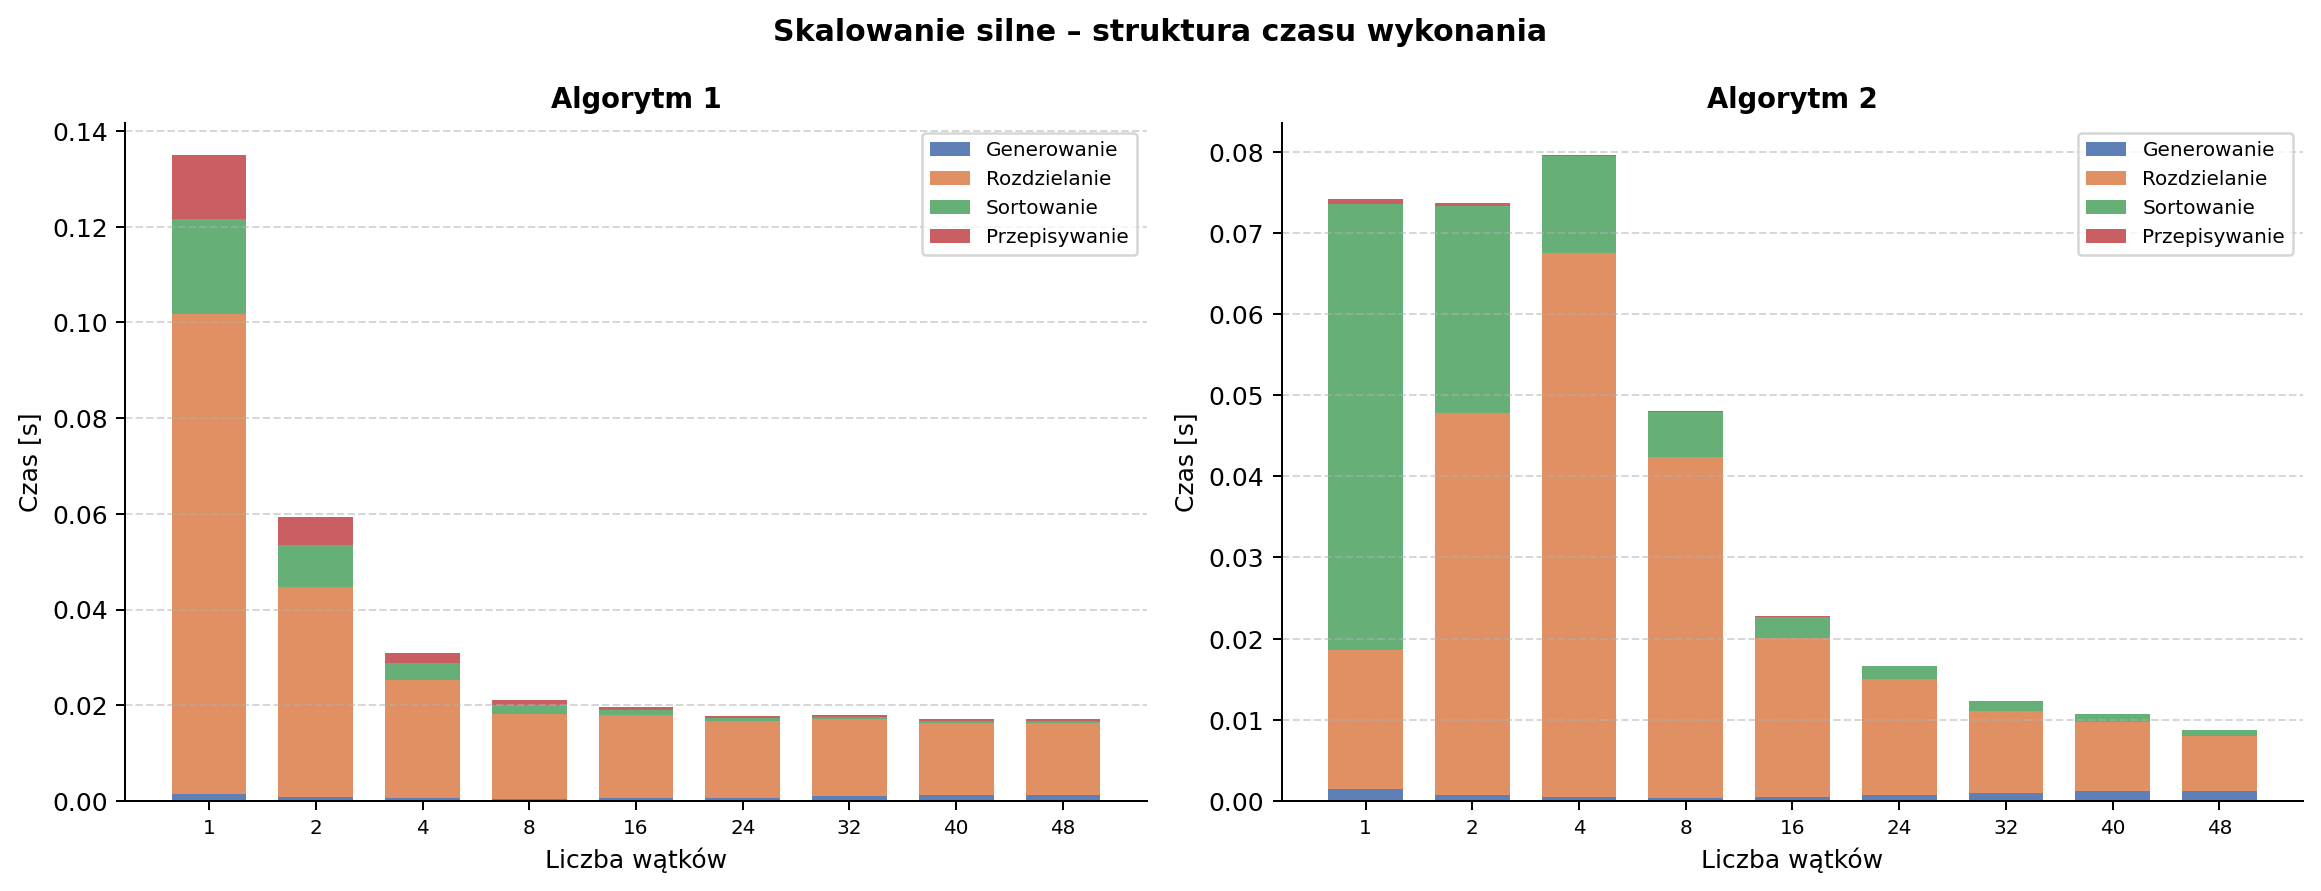
\includegraphics[width=0.72\linewidth]{wykresy/strong_stacked_phases.png}
  \caption{Struktura czasu wykonania — wykres słupkowy skumulowany
           (skalowanie silne, $N=10^6$).}
  \label{fig:strong_stacked}
\end{figure}

\begin{figure}[H]
  \centering
  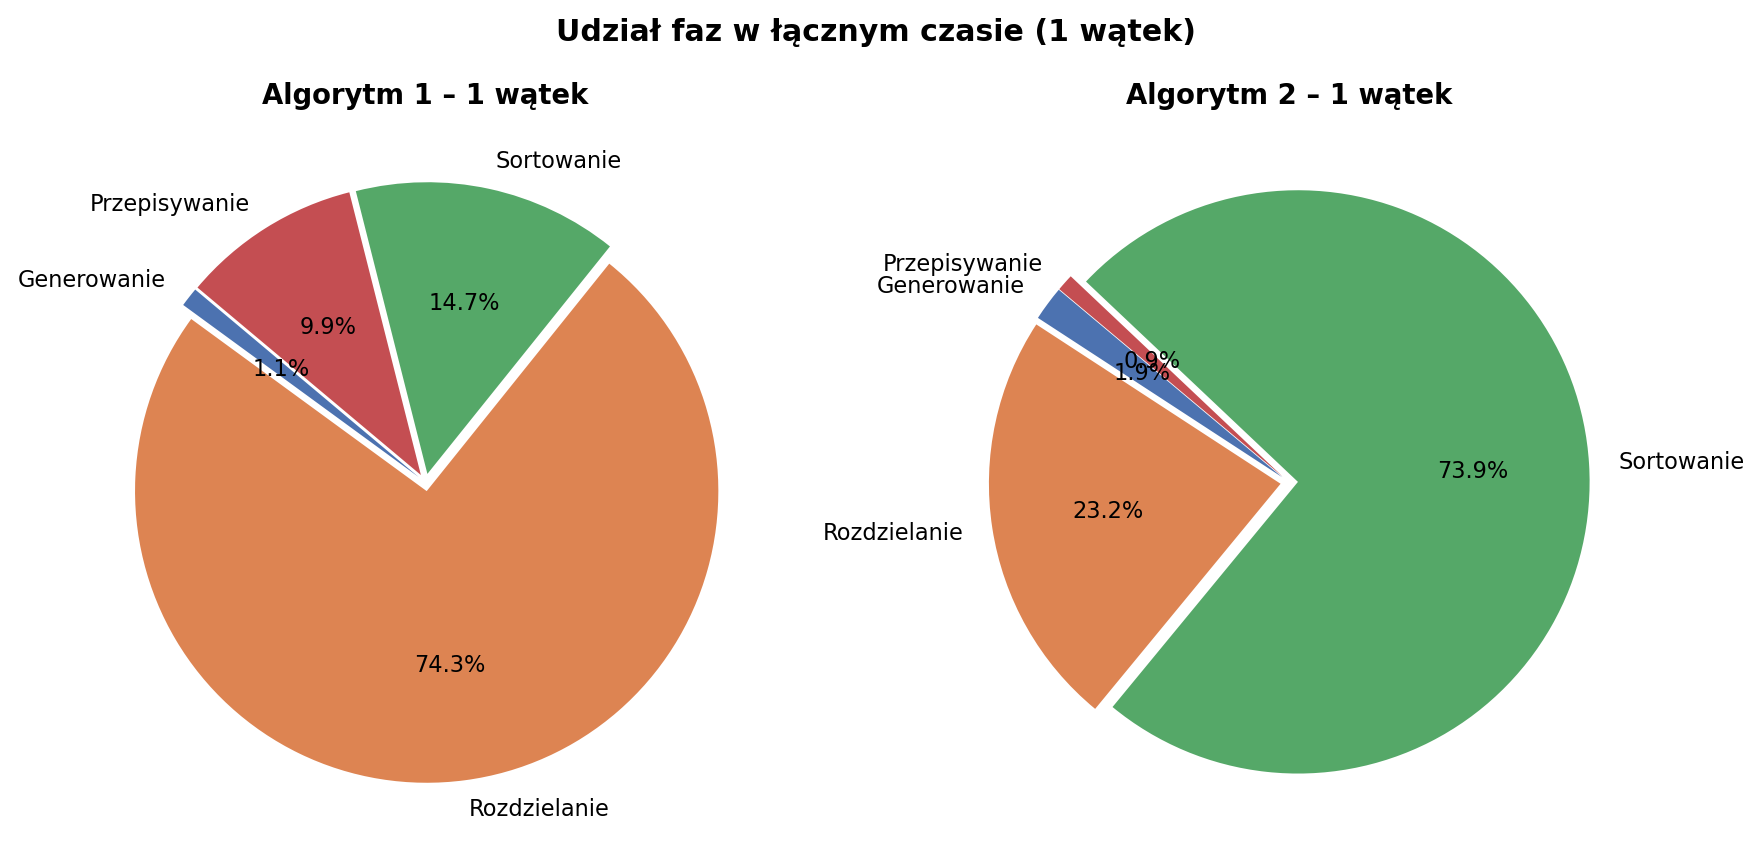
\includegraphics[width=0.65\linewidth]{wykresy/phase_pie_1thread.png}
  \caption{Udział procentowy faz w łącznym czasie wykonania dla 1 wątku.}
  \label{fig:pie}
\end{figure}

Dla \textbf{Algorytmu 1} przy jednym wątku faza rozdzielania dominuje
($\approx\!72\%$ czasu łącznego), a sortowanie kubełków odpowiada za kolejne
$\approx\!14\%$.
Wraz ze wzrostem liczby wątków czas rozdzielania spada szybko, każdy wątek
przetwarza tę samą tablicę, ale jednocześnie.
Ponieważ jednak praca jest nadmiarowa ($O(N\cdot p)$ łącznie), korzyść
z równoległości spłaszcza się powyżej 8~wątków.

Dla \textbf{Algorytmu 2} przy jednym wątku faza sortowania jest najdłuższa
($\approx\!77\%$), a rozdzielanie zajmuje tylko $\approx\!22\%$.
Przy 2–4 wątkach czas \emph{rośnie} względem 1~wątku — jest to efekt
rywalizacji na sekcjach krytycznych w fazie rozdzielania.

\subsubsection{Przyspieszenie}

\begin{figure}[H]
  \centering
  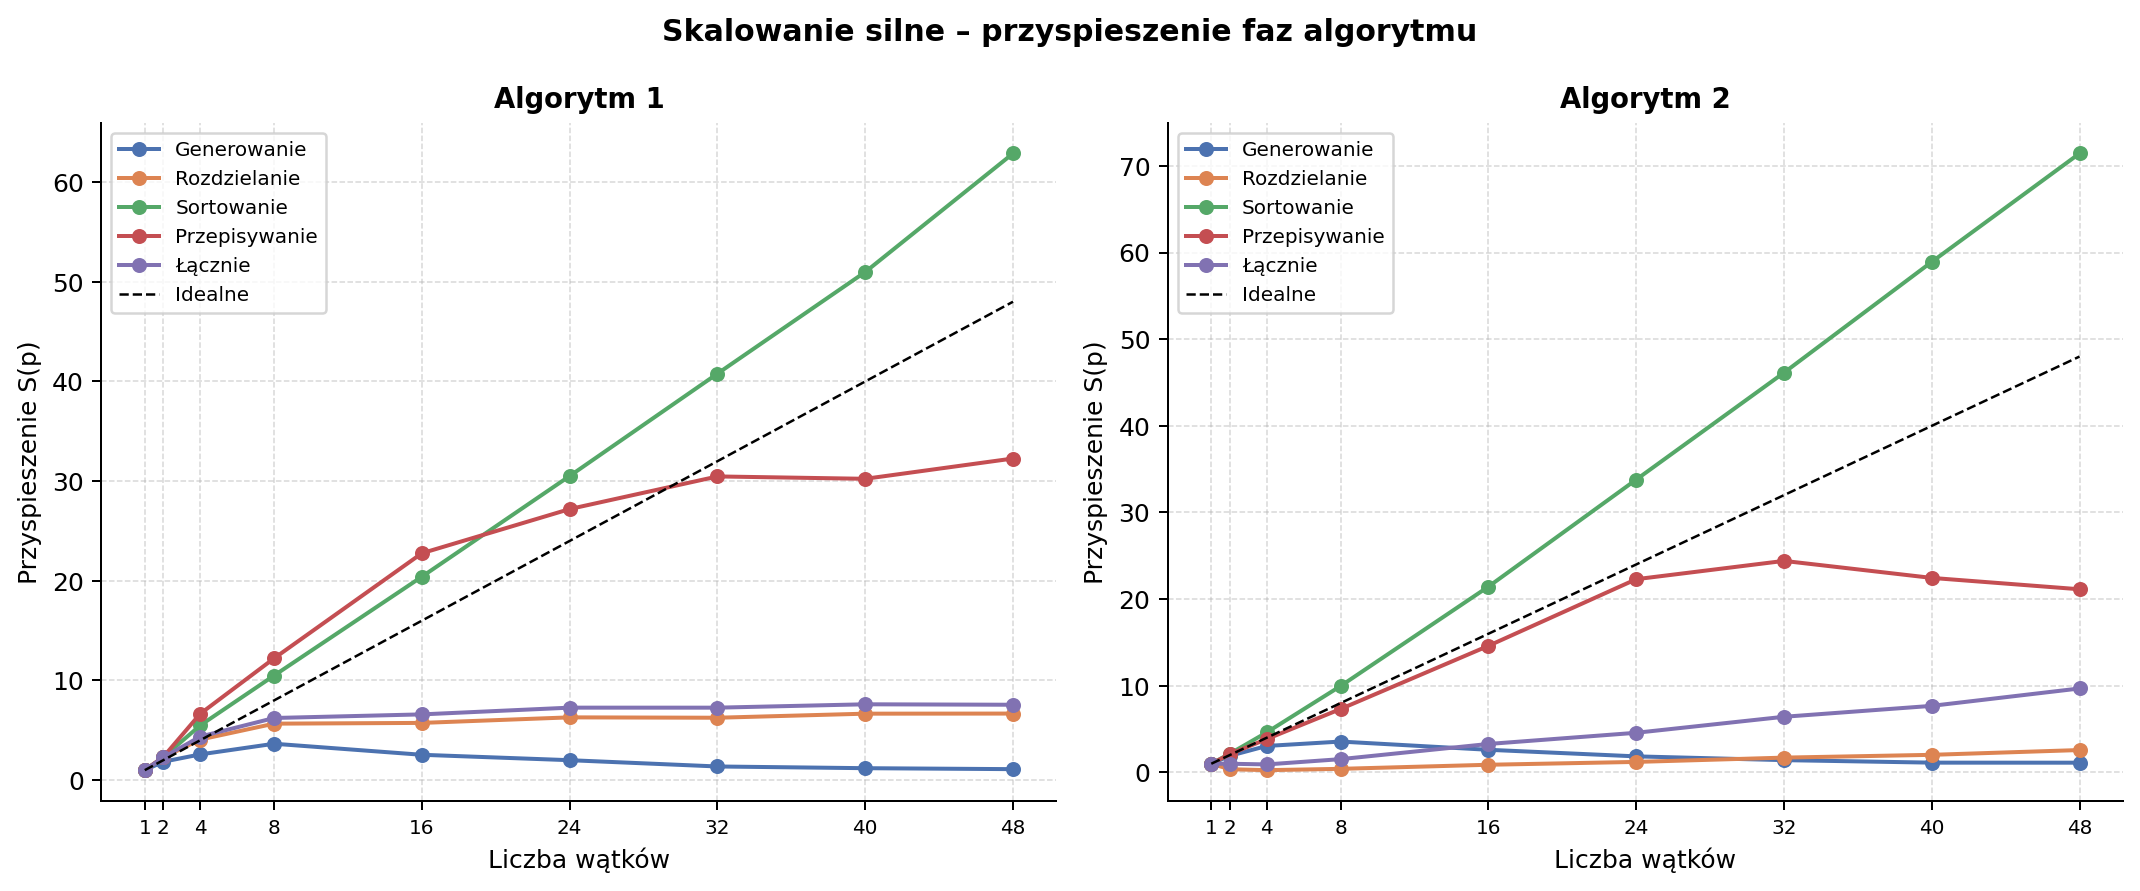
\includegraphics[width=0.85\linewidth]{wykresy/strong_speedup_phases.png}
  \caption{Przyspieszenie poszczególnych faz (skalowanie silne).}
  \label{fig:strong_speedup_phases}
\end{figure}

\begin{figure}[H]
  \centering
  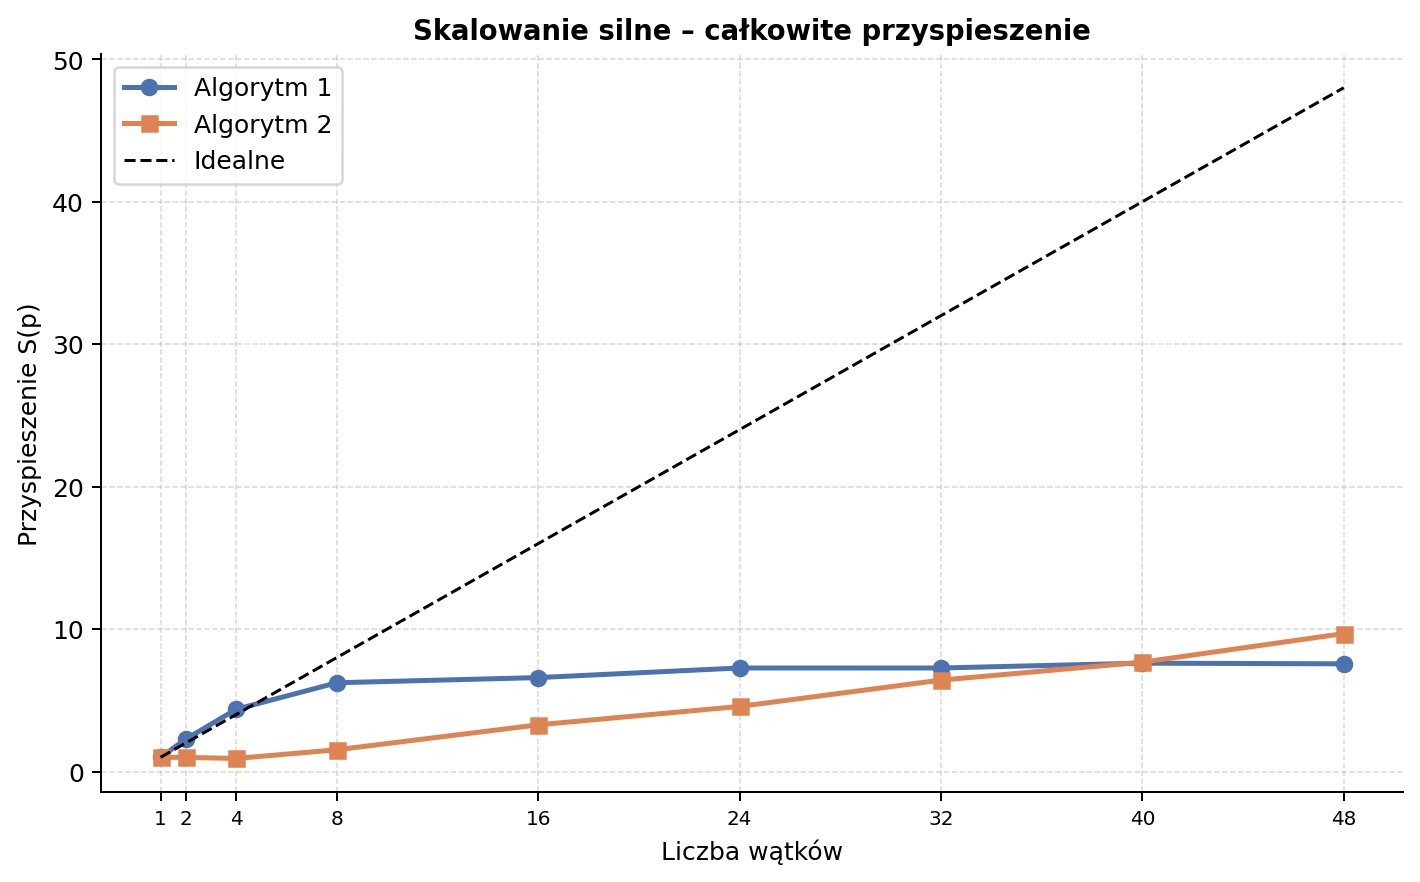
\includegraphics[width=0.65\linewidth]{wykresy/strong_speedup_total.png}
  \caption{Całkowite przyspieszenie obu algorytmów (skalowanie silne).}
  \label{fig:strong_speedup_total}
\end{figure}

\begin{table}[H]
  \centering
  \caption{Całkowite przyspieszenie $S(p) = T(1)/T(p)$ i efektywność $E(p) = S(p)/p$
           dla skalowania silnego.}
  \label{tab:speedup_strong}
  \begin{tabular}{r rr rr}
    \toprule
    & \multicolumn{2}{c}{\textbf{Algorytm 1}} & \multicolumn{2}{c}{\textbf{Algorytm 2}} \\
    \cmidrule(lr){2-3}\cmidrule(lr){4-5}
    \textbf{Wątki} & $S(p)$ & $E(p)$ [\%] & $S(p)$ & $E(p)$ [\%] \\
    \midrule
     1  & 1{,}00 & 100{,}0 & 1{,}00 & 100{,}0 \\
     2  & 2{,}24 & 112{,}2 & 0{,}77 &  38{,}7 \\
     4  & 4{,}34 & 108{,}5 & 0{,}57 &  14{,}2 \\
     8  & 6{,}11 &  76{,}4 & 0{,}75 &   9{,}4 \\
    16  & 6{,}72 &  42{,}0 & 1{,}24 &   7{,}7 \\
    24  & 7{,}13 &  29{,}7 & 1{,}52 &   6{,}3 \\
    32  & 7{,}18 &  22{,}4 & 1{,}74 &   5{,}4 \\
    40  & 7{,}57 &  18{,}9 & 1{,}91 &   4{,}8 \\
    48  & 7{,}35 &  15{,}3 & 2{,}30 &   4{,}8 \\
    \bottomrule
  \end{tabular}
\end{table}

\paragraph{Algorytm 1.}
Przyspieszenie przy 2 i 4 wątkach jest \emph{nadliniowe} ($S(2)=2{,}24$,
$S(4)=4{,}34$).
Wynika to z efektów pamięci podręcznej: dane każdego wątku mieszczą się
w L2/L3, co redukuje liczbę chybień względem sekwencyjnego wykonania.
Powyżej 8~wątków przyspieszenie plateau na poziomie $\approx\!7{,}5\times$
— zgodnie z prawem Amdahla sekwencyjna część programu (generowanie, finalne
przepisywanie) ogranicza dalszy wzrost.

\paragraph{Algorytm 2.}
Przyspieszenie poniżej jedności przy $p<8$ oznacza, że wersja równoległa jest
\emph{wolniejsza} od sekwencyjnej.
Sekcje krytyczne w fazie rozdzielania tworzą wąskie gardło — wątki kolejkują
się do dostępu do każdego kubełka, a narzut synchronizacji przewyższa zysk
z równoległości.
Dopiero przy $p \ge 16$ czas spada poniżej $T(1)$, a maksymalne przyspieszenie
$S(48)=2{,}30$ jest wciąż dalekie od ideału.

% ── Skalowanie słabe ────────────────────────────────────────────────────────
\subsection{Wyniki — skalowanie słabe}

\begin{figure}[H]
  \centering
  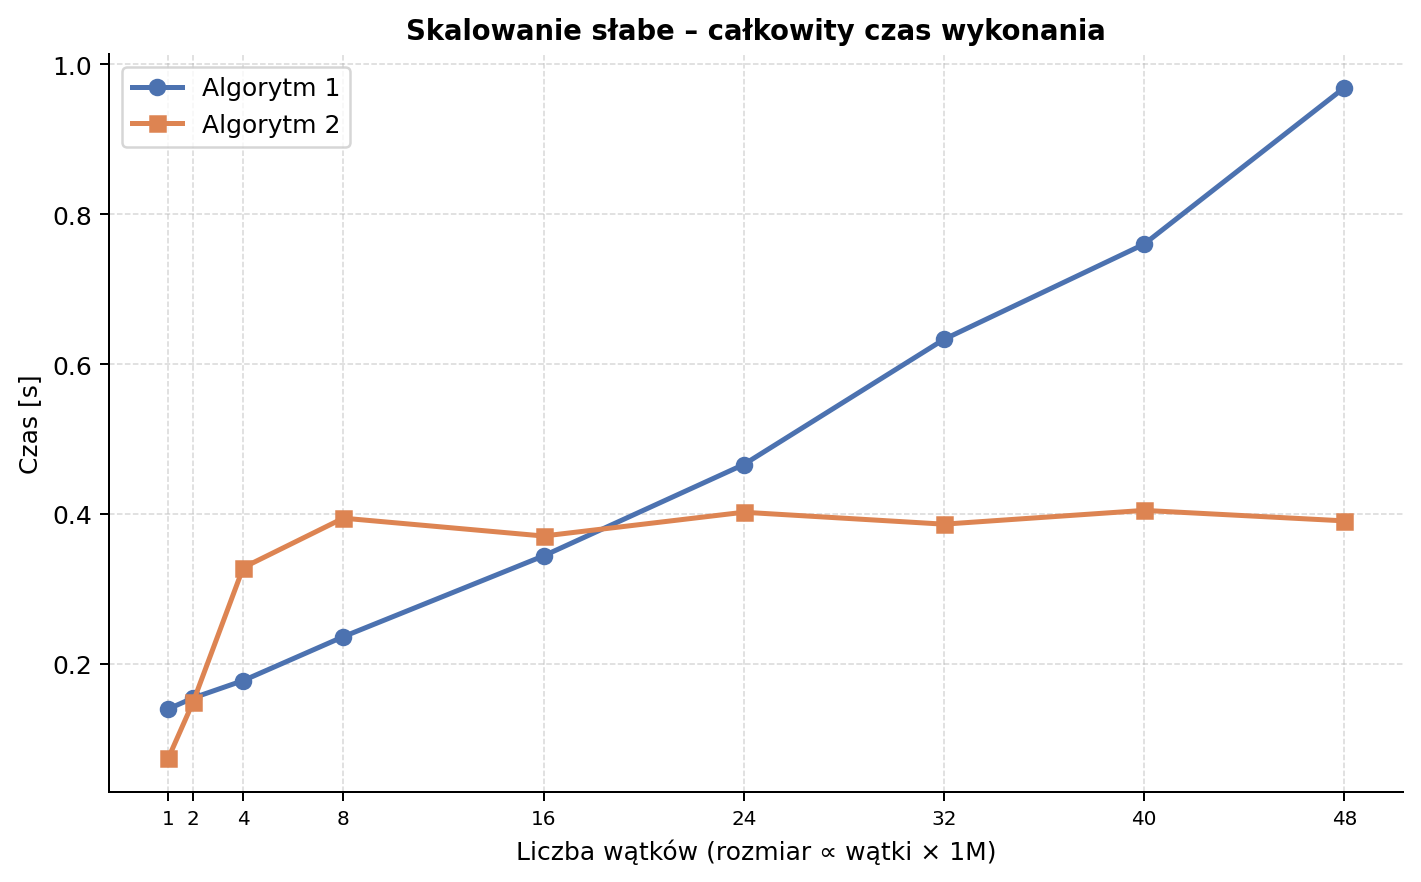
\includegraphics[width=0.72\linewidth]{wykresy/weak_total_comparison.png}
  \caption{Całkowity czas wykonania (skalowanie słabe, $N = p\times 10^6$).}
  \label{fig:weak_total}
\end{figure}

\begin{figure}[H]
  \centering
  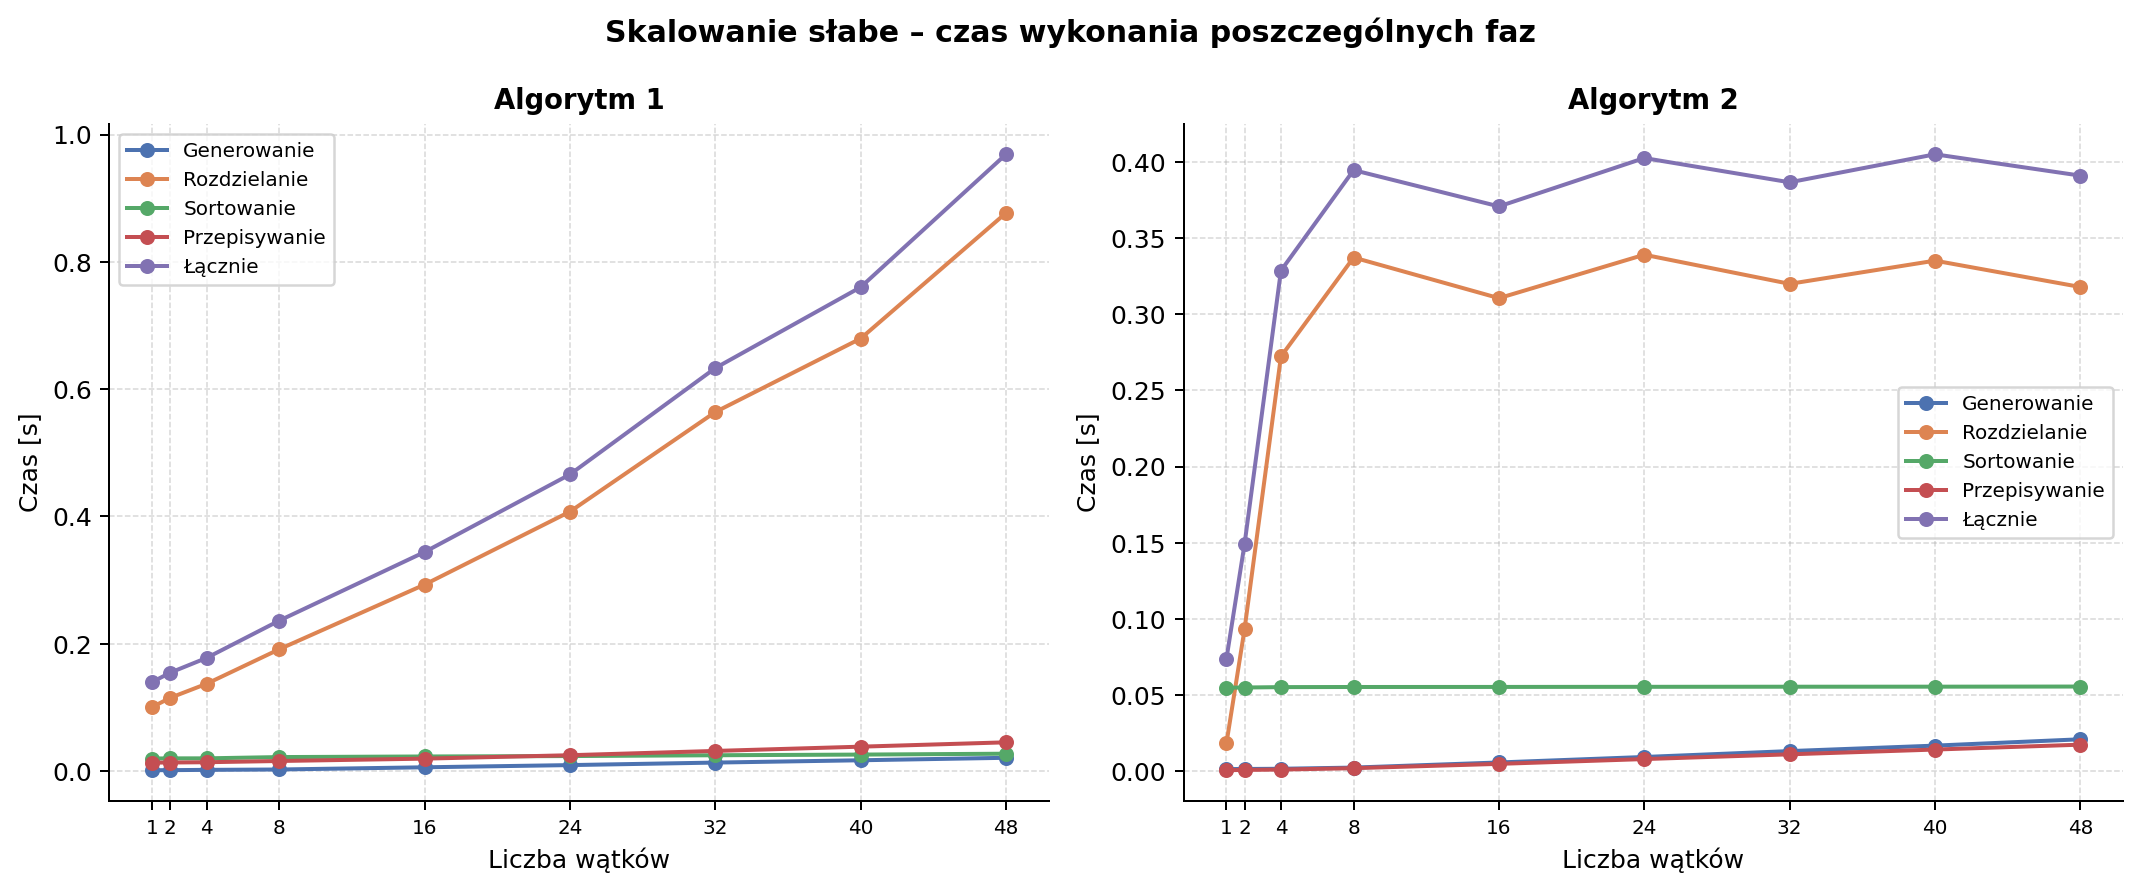
\includegraphics[width=0.85\linewidth]{wykresy/weak_time_phases.png}
  \caption{Czas poszczególnych faz (skalowanie słabe).}
  \label{fig:weak_phases}
\end{figure}

\begin{table}[H]
  \centering
  \caption{Czas łączny i efektywność skalowania słabego
           $E_\text{weak}(p) = T(1)/T(p)\cdot 100\%$.}
  \label{tab:weak}
  \begin{tabular}{r rr rr}
    \toprule
    & \multicolumn{2}{c}{\textbf{Algorytm 1}} & \multicolumn{2}{c}{\textbf{Algorytm 2}} \\
    \cmidrule(lr){2-3}\cmidrule(lr){4-5}
    \textbf{Wątki} & $T(p)$ [s] & $E_\text{weak}$ [\%]
                   & $T(p)$ [s] & $E_\text{weak}$ [\%] \\
    \midrule
     1  & 0{,}139 & 100{,}0 & 0{,}091 & 100{,}0 \\
     2  & 0{,}156 &  89{,}2 & 0{,}235 &  38{,}5 \\
     4  & 0{,}177 &  78{,}4 & 0{,}646 &  14{,}0 \\
     8  & 0{,}238 &  58{,}3 & 0{,}976 &   9{,}3 \\
    16  & 0{,}341 &  40{,}7 & 1{,}228 &   7{,}4 \\
    24  & 0{,}467 &  29{,}8 & 1{,}479 &   6{,}1 \\
    32  & 0{,}630 &  22{,}1 & 1{,}756 &   5{,}2 \\
    40  & 0{,}757 &  18{,}4 & 1{,}969 &   4{,}6 \\
    48  & 0{,}960 &  14{,}5 & 2{,}027 &   4{,}5 \\
    \bottomrule
  \end{tabular}
\end{table}

W \textbf{Algorytmie 1} czas rośnie monotonicznie z $p$, co wynika z rosnącego
całkowitego odczytu ($p$~wątków × $N\cdot p$ elementów).
Efektywność skalowania słabego spada do $14{,}5\%$ przy 48~wątkach.

W \textbf{Algorytmie 2} czas rośnie dramatycznie już przy małej liczbie wątków
($+610\%$ przy przejściu $1\to 4$), po czym tempo wzrostu maleje.
Efektywność spada do $4{,}5\%$ przy 48~wątkach — najgorsza spośród obu
algorytmów.
Jest to konsekwencja kwadratu interferencji: zarówno rozmiar tablicy rośnie
z~$p$, jak i rywalizacja o zamki narasta z liczbą wątków.

% ── Podsumowanie ────────────────────────────────────────────────────────────
\subsection{Wnioski}

\begin{enumerate}
  \item \textbf{Algorytm 1 skalowalny praktycznie, nieefektywny teoretycznie.}
        Mimo redundantnego odczytu tablicy osiąga przyspieszenie
        $S(8)=6{,}1\times$ z efektywnością $76\%$ — nadliniowe wartości dla
        małej liczby wątków potwierdzają efekty cache.
        Plateu powyżej 8~wątków sygnalizuje, że sekwencyjne fazy (generowanie,
        przepisywanie) stanowią ograniczenie zgodne z prawem Amdahla.

  \item \textbf{Algorytm 2 jest sekwencyjnie efektywny, lecz praktycznie
        nieużywalny.}
        Sekcja krytyczna przy zapisie do kubełka tworzy serializowany odcinek
        proporcjonalny do $N/B$ na wątek; przy dużej liczbie wątków koszt
        synchronizacji całkowicie pochłania zysk z równoległości.
        Maksymalne przyspieszenie $S(48)=2{,}30$ jest mniejsze niż
        $S(4)=4{,}34$ Algorytmu~1.

  \item \textbf{Skalowanie słabe jest złe dla obu algorytmów,}
        lecz z różnych przyczyn: w Alg.~1 — rosnący nadmiar pracy;
        w Alg.~2 — narastająca rywalizacja na zamkach.
\end{enumerate}

\end{document}ß
